\documentclass[tikz,border=15pt]{standalone}
\usepackage{amsmath,amssymb}

\begin{document}
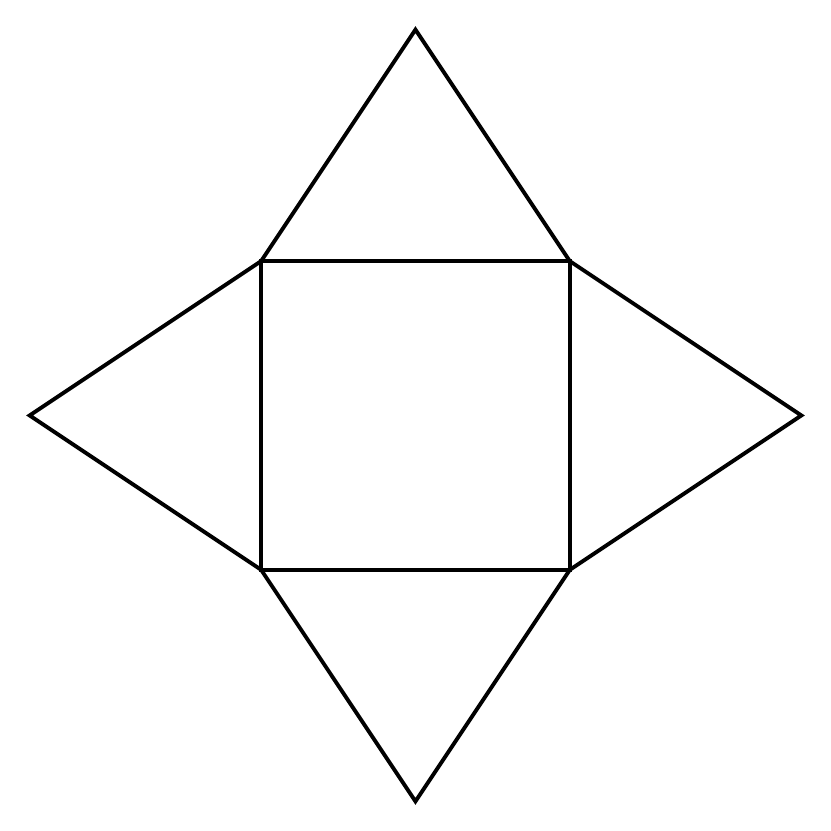
\begin{tikzpicture}[scale=1.4]
    % Regular Square Pyramid Net: square base with 4 congruent isosceles triangles
    \def\s{1.4} % half side of square, side length = 2.8 cm
    \def\htri{2.1} % altitude of the 4 congruent triangular faces
    
    \coordinate (BL) at (-\s, -\s);
    \coordinate (BR) at (\s, -\s);
    \coordinate (TR) at (\s, \s);
    \coordinate (TL) at (-\s, \s);
    
    % Draw central square base
    \draw[line width=1.4pt] (BL) -- (BR) -- (TR) -- (TL) -- cycle;
    
    % 4 symmetric apex points
    \coordinate (ApexTop) at (0, {\s + \htri});
    \coordinate (ApexBot) at (0, {-\s - \htri});
    \coordinate (ApexRight) at ({\s + \htri}, 0);
    \coordinate (ApexLeft) at ({-\s - \htri}, 0);
    
    % Draw 4 congruent triangular faces
    \draw[line width=1.4pt] (TL) -- (ApexTop) -- (TR);
    \draw[line width=1.4pt] (BL) -- (ApexBot) -- (BR);
    \draw[line width=1.4pt] (TR) -- (ApexRight) -- (BR);
    \draw[line width=1.4pt] (TL) -- (ApexLeft) -- (BL);
    
\end{tikzpicture}
\end{document}
